%
% Author: Kian Ho <hui.kian.ho@gmail.com>
%
% Description:
%
%   Seminar slides for introducing COMBINE, who we are, our aims, and events.
%   You could also print these slides and pin them up at conferences as a quick
%   alternative to a proper flyer or poster.
%
% Compilation:
%
%   Latex, beamer, and 'scons' need to be installed, which is easily done using
%   modern Linux distributions such as Ubuntu. SCons automatically handles the
%   latex dependencies during compilation.
%
%   Run 'make' to compile the slides, this in-turn calls 'scons', but you need
%   to ensure that the necessary latex packages are installed. You can do this
%   by searching for the packages named in the '\usepackage{...}' commands in
%   the preamble.
%
%   Run 'make clean' to delete all the latex-generated files prior to a fresh
%   re-compilation.
%

\documentclass[svgnames]{beamer}
\beamertemplatenavigationsymbolsempty
\usetheme{Singapore}

    \makeatletter

    % Change default item bullets from circles to the default triangles. 
    \setbeamertemplate{itemize items}{\raise1.25pt\hbox{\scriptsize$\blacktriangleright$}}

    % Simple footer for each slide showing only the slide number / total slides.
    \setbeamertemplate{footline}
    {
        \begin{minipage}[c]{0.97\paperwidth}
            \raggedleft
            \usebeamerfont{date in head/foot}\usebeamercolor[fg]{title}\insertframenumber{} / \inserttotalframenumber
        \end{minipage}
        \vspace{1.5ex}
    }

\makeatother

\usepackage{varwidth}
\usepackage{xcolor}
\usepackage{graphicx}
\usepackage{hyperref}
\usepackage{verbatim}
\usepackage{varwidth}
\usepackage{microtype}
\usepackage{etoolbox}
\usepackage[export,Export]{adjustbox}

    \providebool{longversion}
    \setbool{longversion}{true}

    \newcommand{\beamerpurple}[1]{{\usebeamercolor[fg]{title}#1}}
    \newcommand{\bp}[1]{{\usebeamercolor[fg]{title}#1}}
\begin{document}

\begin{frame}
    \centering
    \vfill
    {\LARGE \bp{\bfseries COMBINE Student Symposium 2013}}\\[1ex]
    \href{http://www.combine.org.au}{\bp{www.combine.org.au}}\\[2ex]
    {November 28, 2013}\\
    \vfill
    \begin{minipage}[c]{\linewidth}
        \centering
        sponsored by:\\
        
\includegraphics[height=10mm,valign=T]{./images/logo_vlsci_3508x1890.jpg}
        \qquad
        
\includegraphics[height=10mm,valign=T]{./images/ICT-for-Life-Sciences-Forum-logo.png}
        \qquad
        
\includegraphics[height=10mm,valign=T]{./images/nicta_logo.png}
    \end{minipage}
\end{frame}

\begin{frame}{Program}
    \centering
    \begin{minipage}[c]{0.8\linewidth}
        \begin{itemize}
            \item[11:00am] Registration \& Morning Tea
            \item[11:30am] Welcome \& Introduction to COMBINE
            \item[11:40am] \textbf{Oral Presentations} (Session 1)
            \item[1:00pm] Break - Lunch
            \item[2:00pm] \textbf{Oral Presentations} (Session 2)
            \item[3:00pm] Break - Afternoon Tea
            \item[3:30pm] \textbf{Careers Panel Q\&A} (chair: Prof.~Chris Leckie)
            \item[4:30pm] Awards \& Symposium Close
            \item[5:00pm] Social Event
        \end{itemize}
    \end{minipage}
\end{frame}

\begin{frame}
    \vfill
    \begin{minipage}[c]{\linewidth}
        \centering
        
\includegraphics[width=0.5\linewidth]{./images/COMBINE-logo.png}
    \end{minipage}
    \vfill
    \beamerpurple{COMBINE} is a student-run Australian organisation for researchers in
    \textbf{computational biology}, \textbf{bioinformatics}, and related
    fields.\\[2ex]
    We aim to bring together students and early-career
    researchers from the computational and life sciences for networking,
    collaboration, and professional development.\\[1ex]
    \vfill
\end{frame}

\begin{frame}{Previous COMBINE Events}
    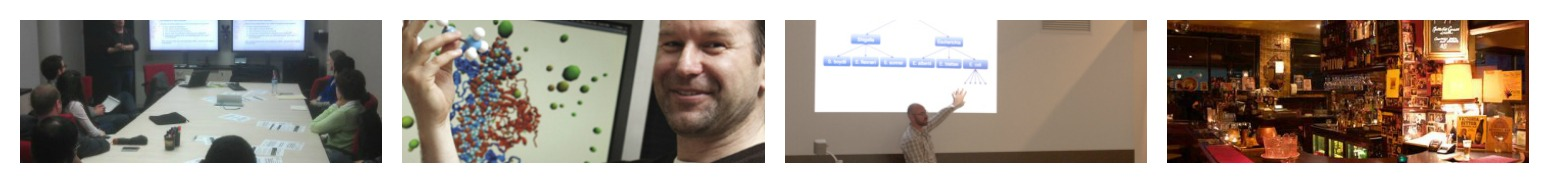
\includegraphics[width=\linewidth]{./images/COMBINE-collage.jpg}
    \vspace{1ex}
    \bp{\bfseries Alignment free methods for sequence comparison} (seminar)\\
    Dr.~Tom Conway, NICTA\\[2ex]
    \bp{\bfseries How to get your computer to freeze} (seminar)\\
    Dr.~Mike Kuiper, VLSCI\\[2ex]
    \bp{\bfseries How to give a better research presentation} (workshop)\\
    Prof. Justin Zobel, Uni.~Melb.\\[2ex]
    \bp{\bfseries Python for the Life Sciences} (workshop)\\
    Dr.~Bernie Pope, VLSCI\\[2ex]
    \bp{\bfseries Wikipedia edit-a-thon \& Pizza Lunch} (workshop/social)\\
    Drs.~Gayle Philip, Bernie Pope, and Geoff Macintyre.
\end{frame}

\ifbool{longversion}{

\begin{frame}

\begin{minipage}[c]{\linewidth}
    \vfill

    \beamerpurple{COMBINE} is the official
    \href{http://www.iscb.org/}{\beamerpurple{ISCB}} Regional Student Group for
    Australia.

    \vspace{3ex}

    \begin{minipage}[c]{\linewidth}
        \centering
    \begin{minipage}[c]{0.47\linewidth}
        \centering
        
\includegraphics[width=0.85\linewidth,valign=M]{./images/iscb_logo.png}\\[1ex]
        
\includegraphics[width=0.85\linewidth,valign=M]{./images/ISCBSC-logo.png}
    \end{minipage}
    ~
    \begin{minipage}[c]{0.33\linewidth}
        \centering
        
\includegraphics[scale=0.12]{./images/RSGAU-logo.png}
    \end{minipage}
    \end{minipage}

    \vspace{3ex}

    \begin{itemize}
        \item ISCB - International Society for Computational Biology
        %\item 25 ISCB Regional Student Groups (RSGs) around the world.
        \item ISMB2014 - July 11--15, 2014 in Boston, USA.
        \item ECCB2014 - September 7--10, 2014 in Strasbourg, France.
    \end{itemize}

    \vfill
\end{minipage}

\end{frame}

}{}

%   \begin{frame}{Previous COMBINE Events}
%       \centering
%       \vfill
%       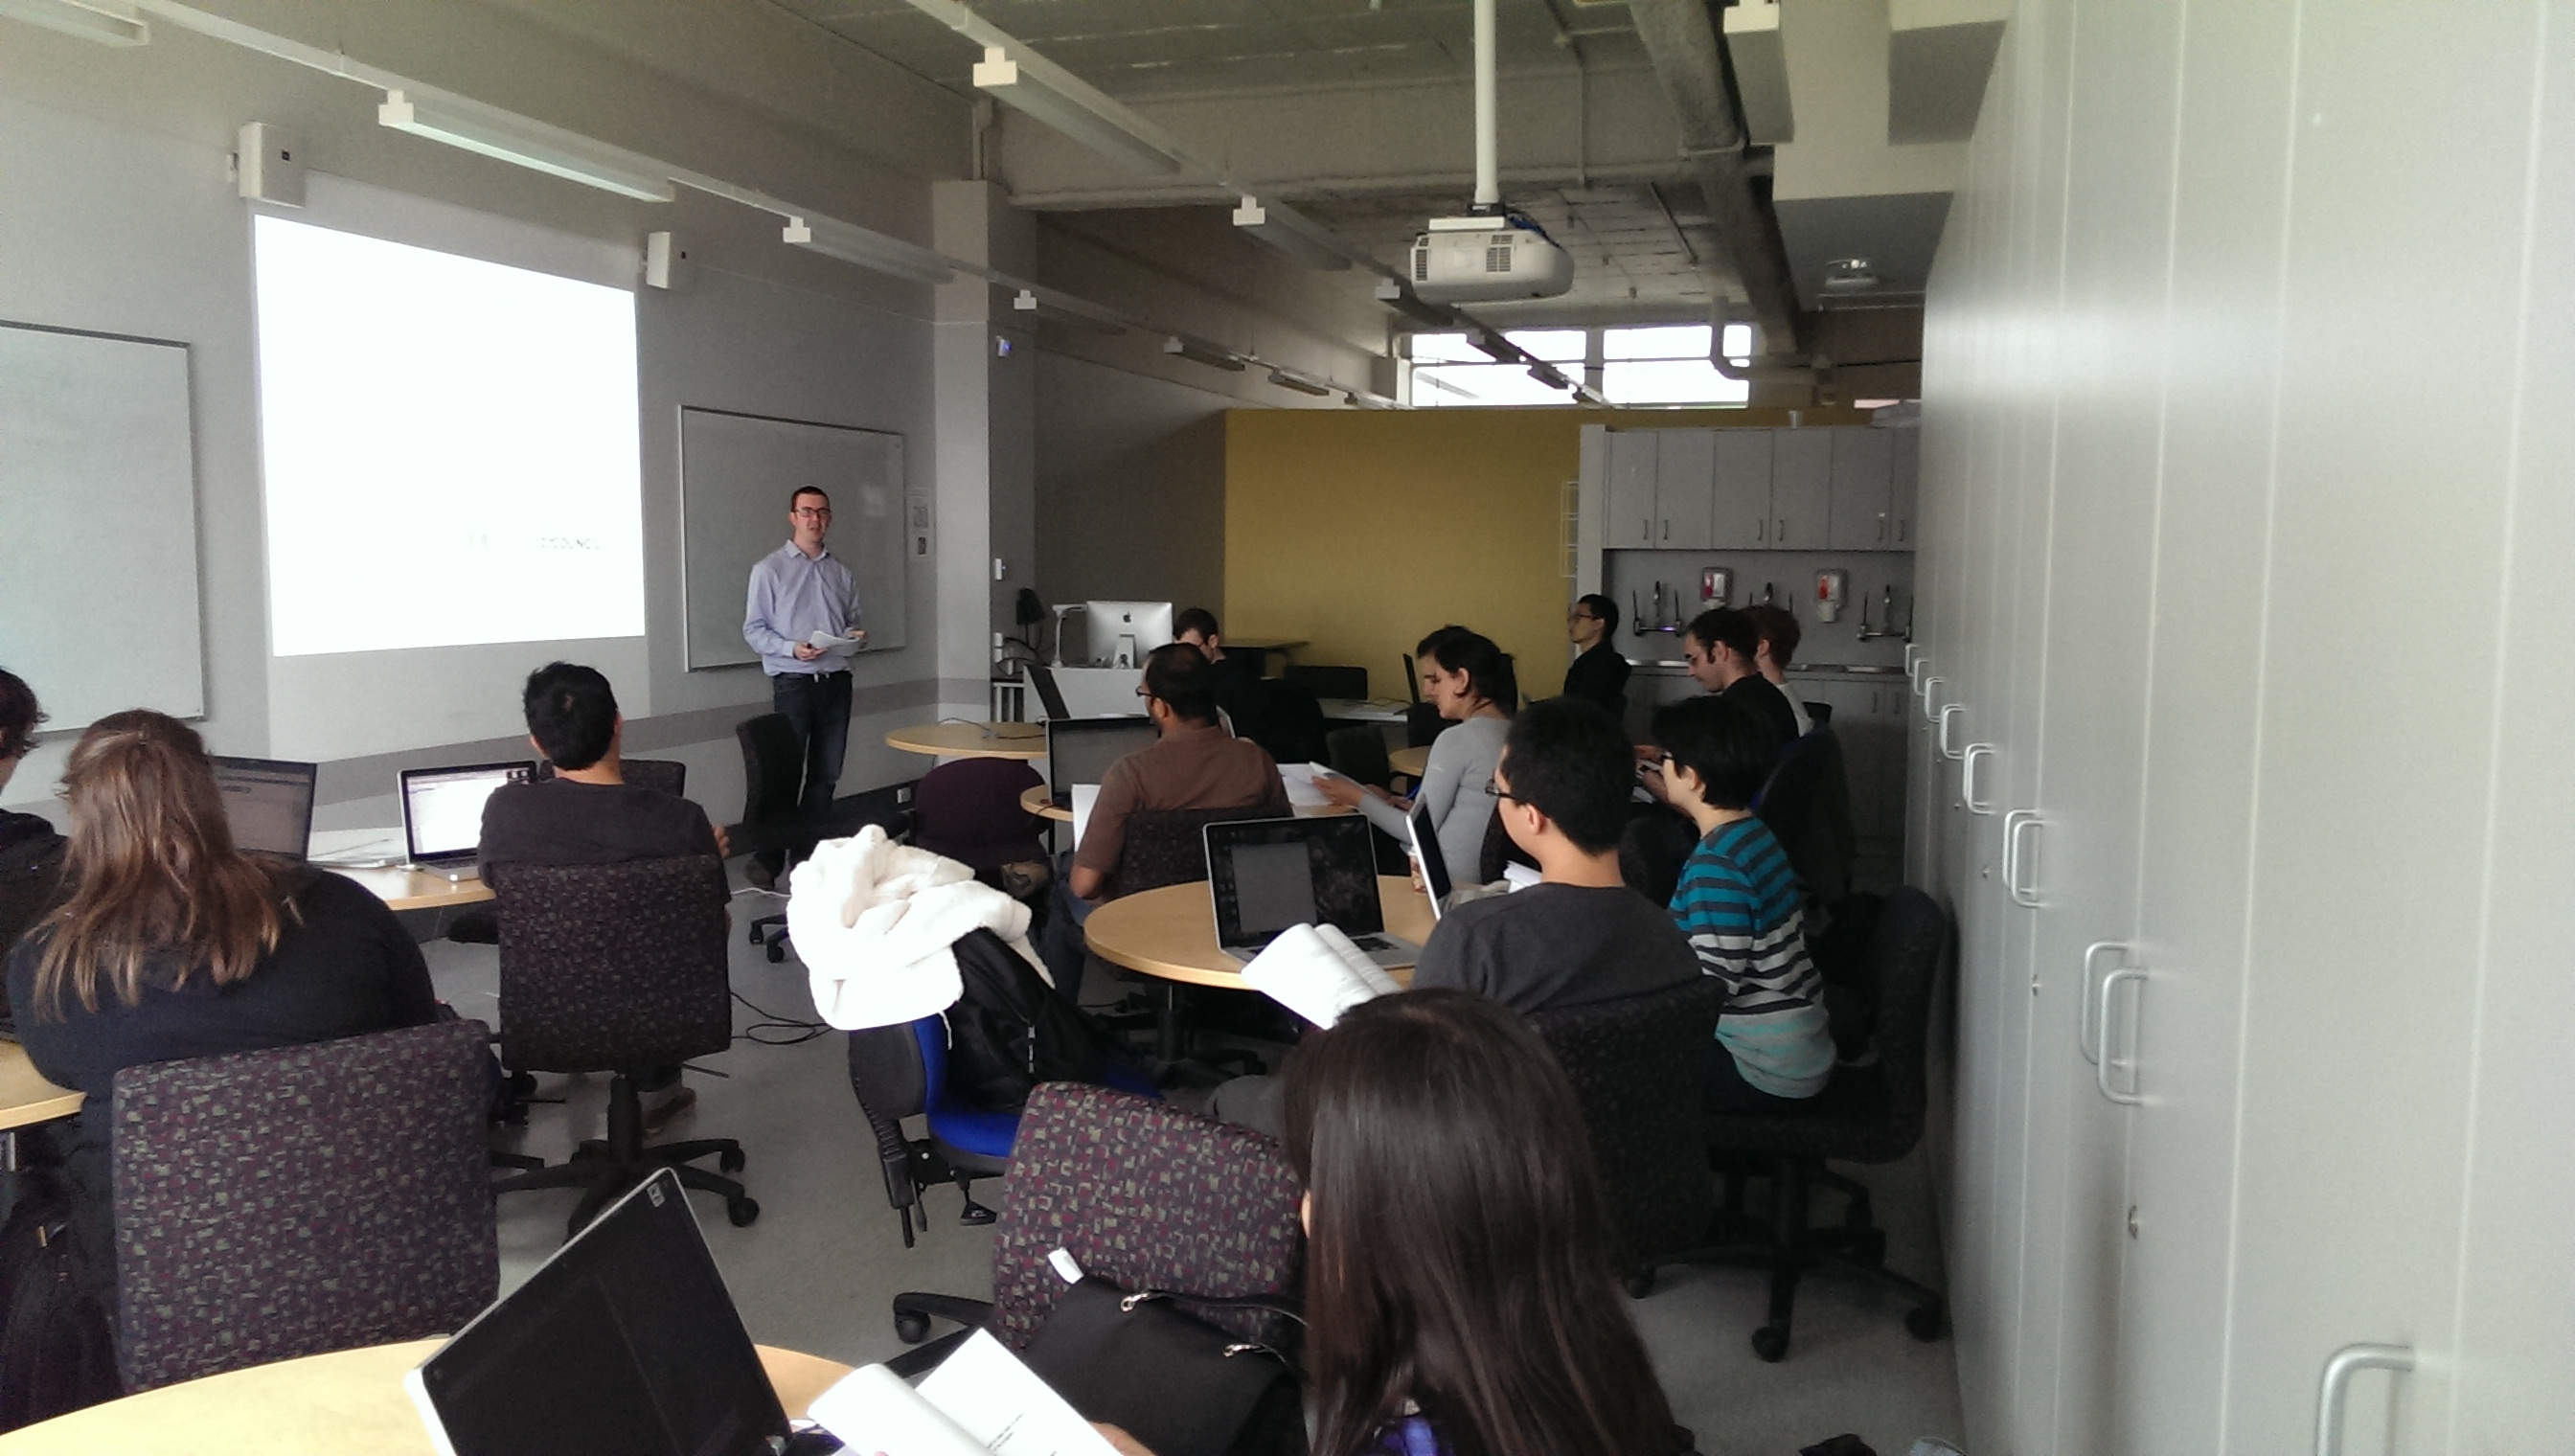
\includegraphics[height=0.6\paperheight]{./images/python-workshop-photo.jpg}\\
%       \textbf{Python Workshop}\\
%       Dr.~Bernie Pope, VLSCI\\[2ex]
%   \end{frame}

%   \begin{frame}{Previous COMBINE Events}
%       \centering
%       \vfill
%       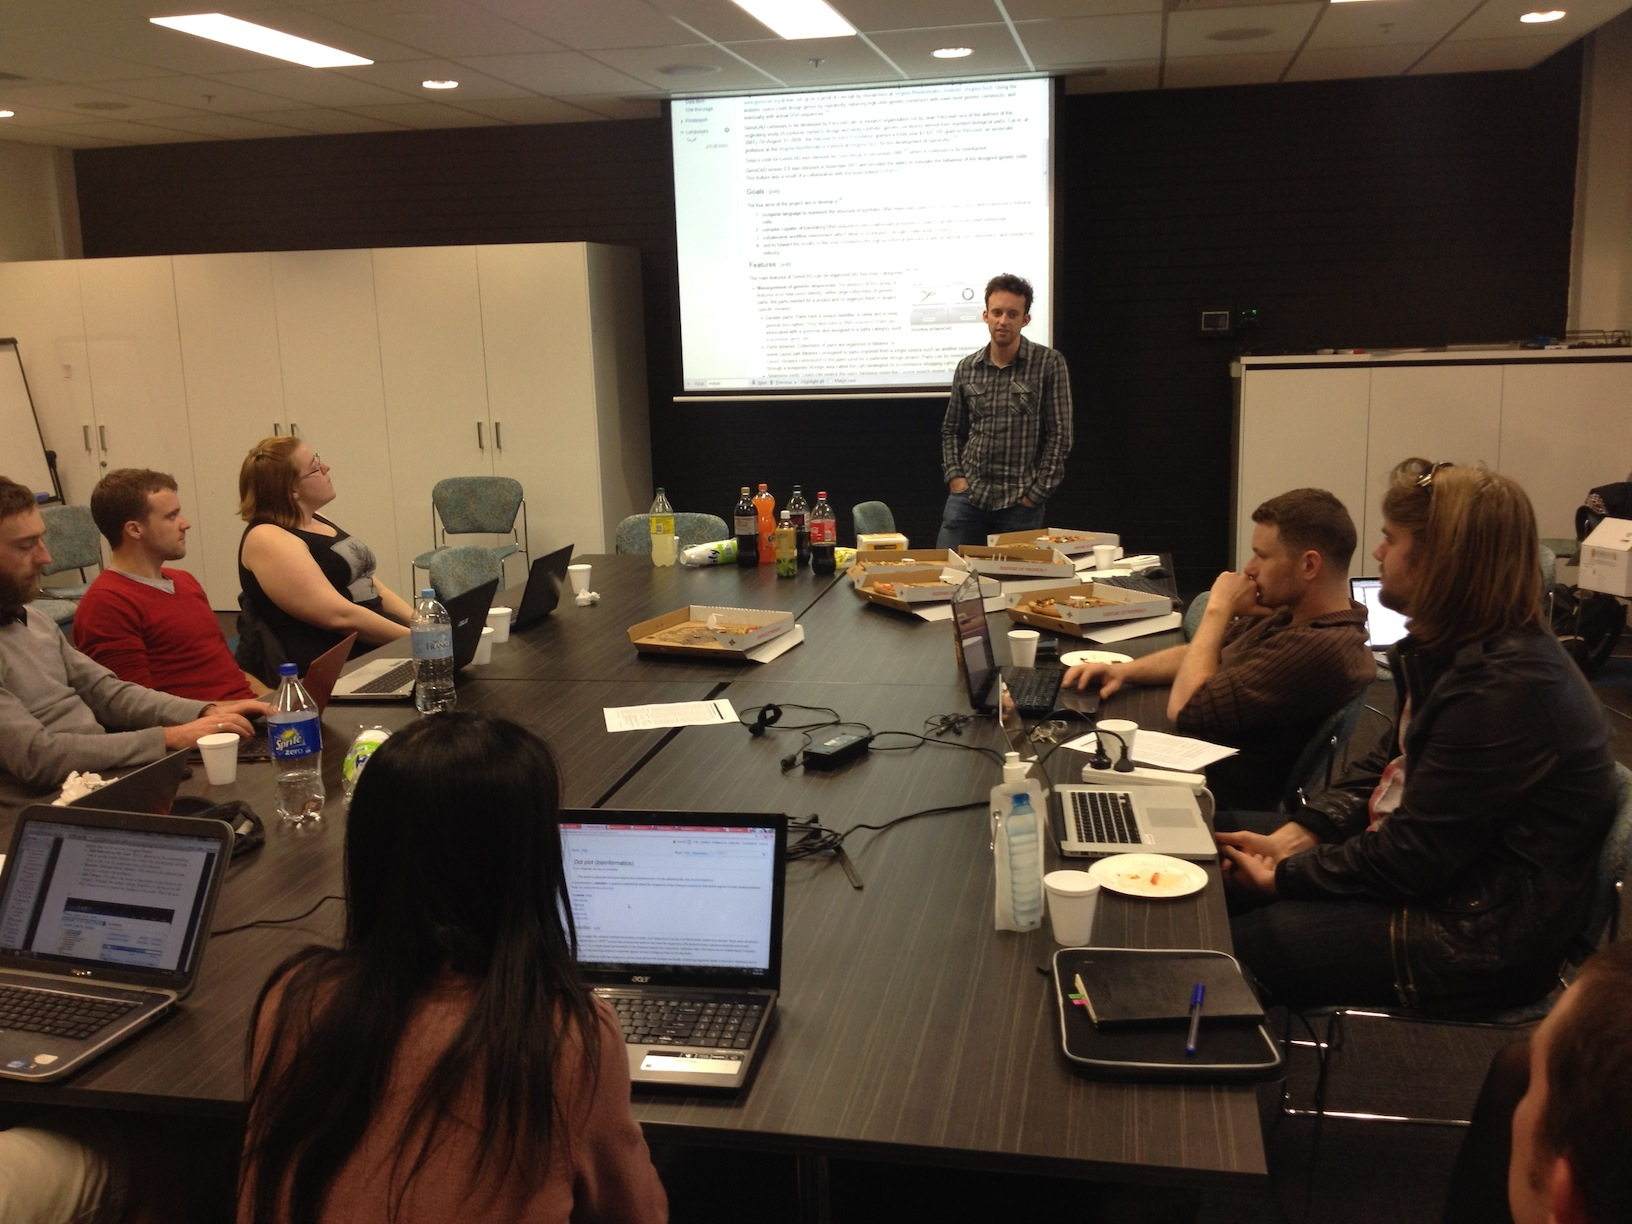
\includegraphics[height=0.7\paperheight]{./images/wikipedia-editathon-photo.jpg}\\
%       \textbf{Wikipedia edit-a-thon \& Pizza Lunch}\\
%   \end{frame}

\begin{frame}{Join Us!}
    \begin{itemize}
        \item We are currently looking for volunteers to join our committee.
        \item Present your work at a COMBINE event before the conferences!
        %\item Are you an expert on $x$? Give a workshop on $x$!
    \end{itemize}

    \vspace{1ex}

    \bp{Our Committee:}\\
        %\item we run seminars, workshops, symposiums, and social events.
        Benjamin Goudey (\emph{President}),
        Karin Klotzbuecher (\emph{Secretary}),
        Sabrina Rodrigues,
        Andrew Lonsdale,
        Thomas Coudrat,
        Kian Ho\\[2ex]

    Email: \bp{combine@combine.org.au}\\
    Mailing list: \bp{combine.org.au/join}\\
    Facebook: \bp{facebook.com/combine.australia}\\
    Twitter: \bp{twitter.com/combine\_au}\\[2ex]
    For more information, visit \beamerpurple{\href{http://www.combine.org.au}{combine.org.au}}\\[2ex]

    
    COMBINE is sponsored by:\quad
    \begin{minipage}[c]{0.2\linewidth}
        \centering
        \href{http://ict4lifesciences.org.au/}
            {
\includegraphics[height=0.1\paperheight]{./images/ICT-for-Life-Sciences-Forum-logo.png}}
    \end{minipage}\quad
    \begin{minipage}[c]{0.25\linewidth}
        \centering
        \href{http://www.iscbsc.org/}{
\includegraphics[height=0.1\paperheight]{./images/ISCBSC-logo.png}}
    \end{minipage}
\end{frame}

\begin{frame}{Remarks}

\textbf{\bp{Dr.~Geoff Macintyre}}
\begin{itemize}
    \item Senior Researcher, NICTA Diagnostic Genomics Group
    \item Former President of the ISCB Student Council and COMBINE.
\end{itemize}
\end{frame}

\end{document}
